\section{Converged Graph Relational Optimization Framework}

\begin{figure}
    \centering
    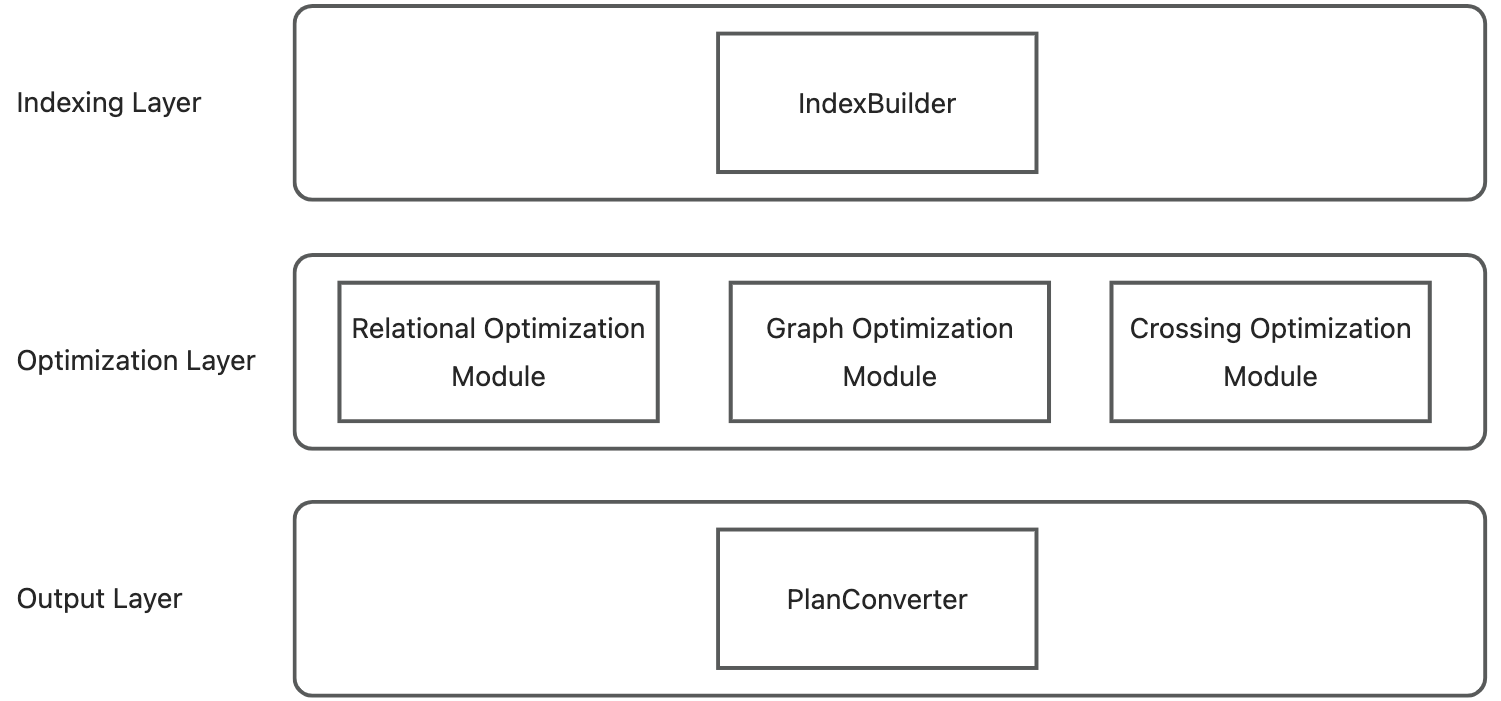
\includegraphics[width=\linewidth]{./figures/framework.png}
    \caption{Overview of the Converged Graph Relational Optimization Framwork.}
    \label{fig:framework-overview}
\end{figure}


To optimize SPJM queries, we propose the converged graph relational optimization framework named relgo.
Specifically, optimizing SPJM queries with relgo is divided into three stages, i.e., preprocessing, optimizing, and converting.
In this section, we introduce the three stages of relgo in detail.

\subsection{Preprocessing Stage}
Given an SPJM query, relgo first parse the query and obtained the corresponding AST (Abstract Syntax Tree).
Then, the initial logical plan is obtained based on the AST.
Each node in the logical plan represents an operator, including the selection, projection, join, and scan operators.

Please note that the matching operator does not appear in logical plans, because it can be further decomposed into other operators such as join and selection operators.
Besides, according to \refdef{matching}, the output of the matching operator is a graph relation, and it is always followed by a projection operator $\widehat{\pi}$.
The output of $\widehat{\pi}$ is a relation and the matching operator as well as $\widehat{\pi}$ are considered as a whole as an implementation of the scan operator (named ScanMatchTable).

In the preprocessing stage, some universally effective optimizations can be applied to refine the plan in advance.
A typical optimization is \filterrule.

This rule is inspired by FilterPushdownRule in relational optimizer, which can push down the predicates to the scan operators to filter out invalid elements earlier.
Specifically, as the ScanMatchTable corresponding to $\matching(\pattern)$ is a physical implementation of the scan operator which acts like scanning a table obtained by matching $\pattern$, it is reasonable to integrate some filtering criteria into the ScanMatchTable operator.
Specifically, \filterrule finds predicates on the properties of elements in $\pattern$ and push them down into ScanMatchTable, so that invalid elements can be dropped earlier.
An example of applying \filterrule is given in Example \ref{example:push_down}.

Formally, the equation rule w.r.t.~\filterrule is as follows:
\begin{equation}
    \begin{split}
        & \pi_A(\sigma_{d}(R_1 \Join \cdots \Join R_m \Join \widetilde{R}) \\
        & \hspace*{2em} \equiv \pi_A(\sigma_{d_0}(R_1 \Join \cdots \Join R_m \Join \widetilde{R}_{d_1})), \\
        & \hspace*{4em} \text{where } \widetilde{R} = \widehat{\pi}_{attr*}(\mathcal{M}(\mathcal{P})) \\
        & \hspace*{4em} \text{and } \widetilde{R}_{d_1} = \widehat{\pi}_{attr*}(\mathcal{M}(\mathcal{P}_{d_1}))
    \end{split}
\end{equation}
where $d_1$ is a subset of $d$ with the constraints related to $\widetilde{R}$ and $d_0$ is obtained by removing $d_1$ from $d$.
Besides, $\mathcal{P}_{d_1}$ is obtained by adding constraints in $d_1$ to $\mathcal{P}$.

\subsection{Optimizing Stage}

Given a logical plan of a SPJM query, relgo optimizes the plan in the optimizing stage.
Specifically, the operations that appear in logical plans of SPJM queries often also appear in the logical plans of relational databases.
Therefore, typical relational optimizers, e.g., Calcite \cite{calcite}, can be employed to optimize this plan.

Besides, to optimize the implementation of ScanMatchTable, the matching plans are optimized with graph-aware methods.
Studies that optimize graph pattern matching can be utilized as the graph-aware methods, and when implementing \name, we leverage GLogS \cite{GLogS} to optimize matching plans.
Moreover, if graph indices are available, join operators in \expandvertex and \expandintersect can be implemented as predefined joins to further improve the efficiency. 


\subsection{Converting Stage}

As different databases usually support different operators and their physical plans can be greatly varied, it is of critical importance for an optimization framework to be flexible.
Therefore, we implement a PlanConverter in the framework to ensure the flexibility.
Given the generated optimal physical plan, the PlanConverter transforms the plan to an internal representation (e.g., Substrait \cite{substrait}), and then the internal representation is transformed to the physical plan that can be executed by the target database.
Finally, the plan is executed and the query results are obtained.


The introduction of the framework is concluded with an example.


\begin{figure}
    \centering
    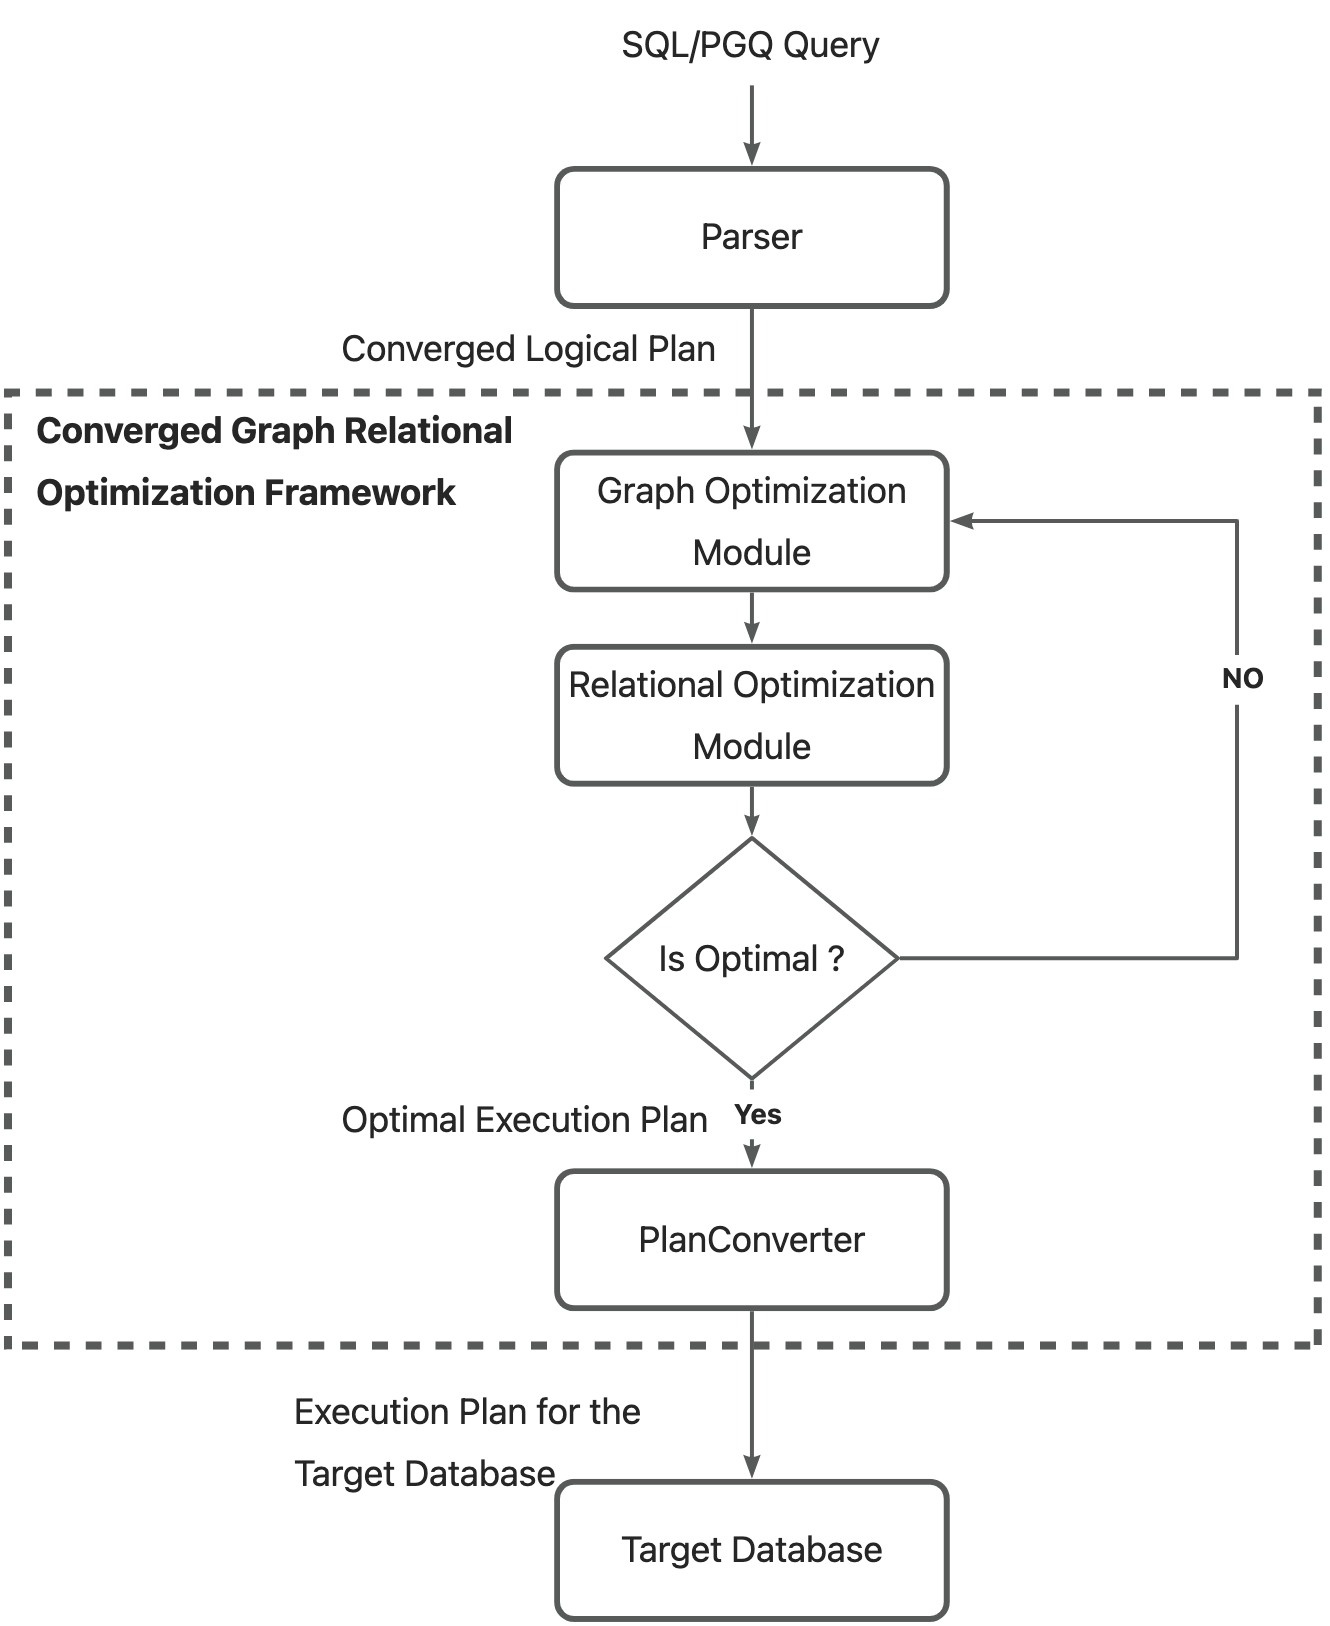
\includegraphics[width=.8\linewidth]{./figures/workflow.png}
    \caption{Workflow of the Converged Graph Relational Optimization Framework.}
    \label{fig:workflow}
\end{figure}

\begin{figure}
    \centering
    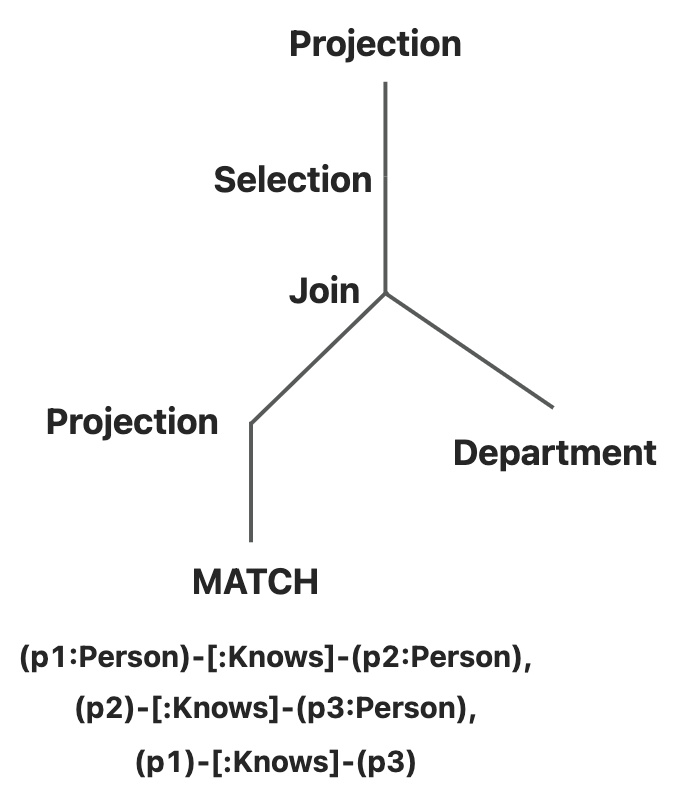
\includegraphics[width=.6\linewidth]{./figures/example_tree.png}
    \caption{The operator tree of SPJM query in Example \ref{example:framework}.}
    \label{fig:example-operator-tree}
\end{figure}

\begin{figure*}
    \centering
    \begin{subfigure}[b]{0.4\linewidth}
        \centering
        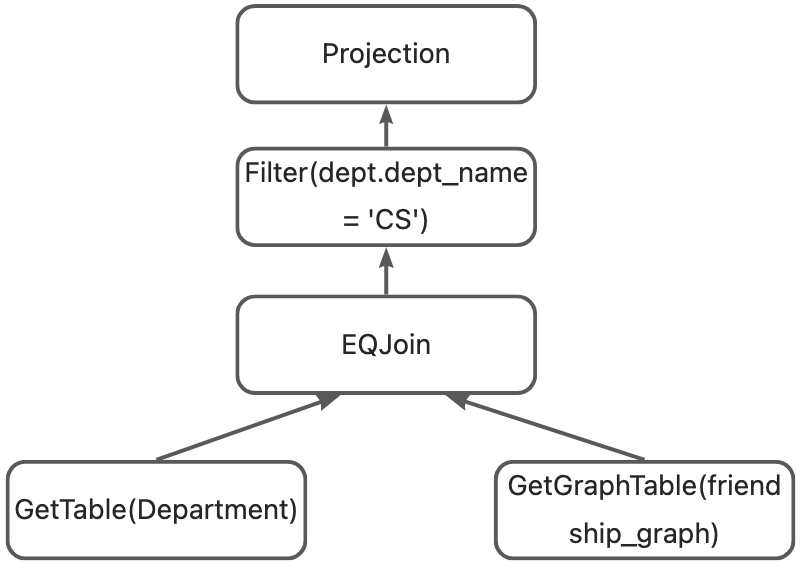
\includegraphics[width=\linewidth]{./figures/converged-logical-plan-relational.png}
        \caption{Outer query plan.}
        \label{fig:converged-logical-plan-relational}
    \end{subfigure}
    \begin{subfigure}[b]{0.4\linewidth}
        \centering
        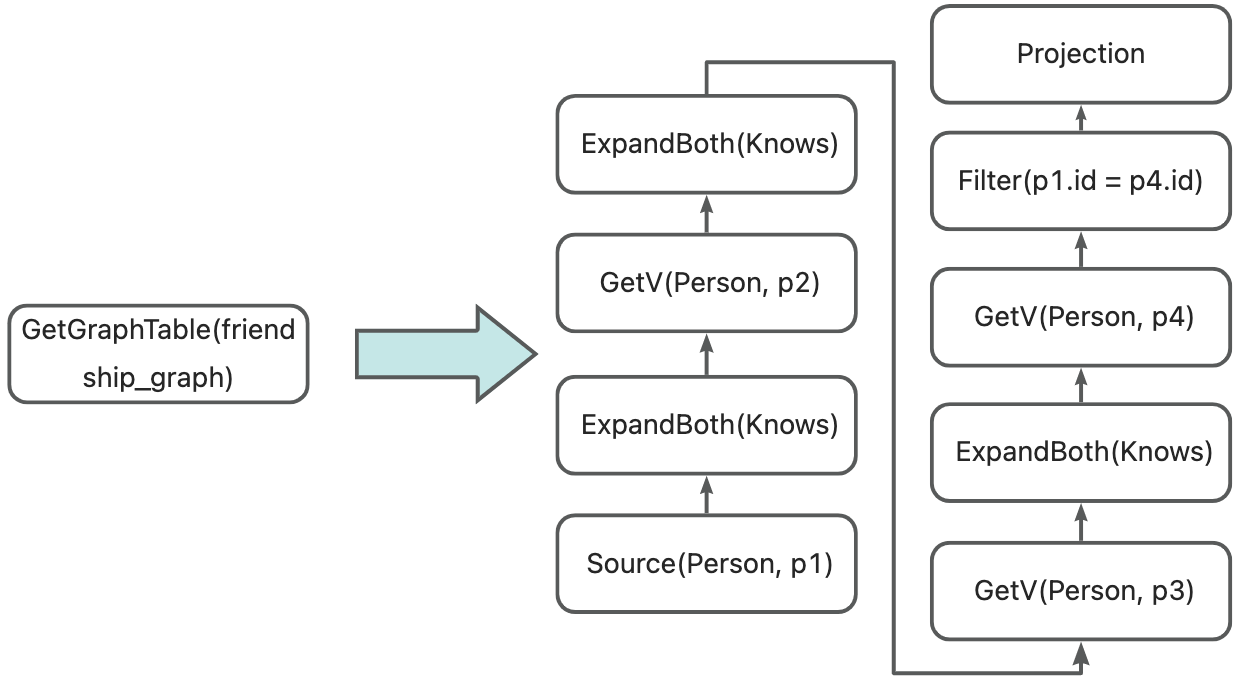
\includegraphics[width=\linewidth]{./figures/converged-logical-plan-graph.png}
        \caption{Match scanning plan.}
        \label{fig:converged-logical-plan-graph}
    \end{subfigure}
    \begin{subfigure}[b]{0.4\linewidth}
        \centering
        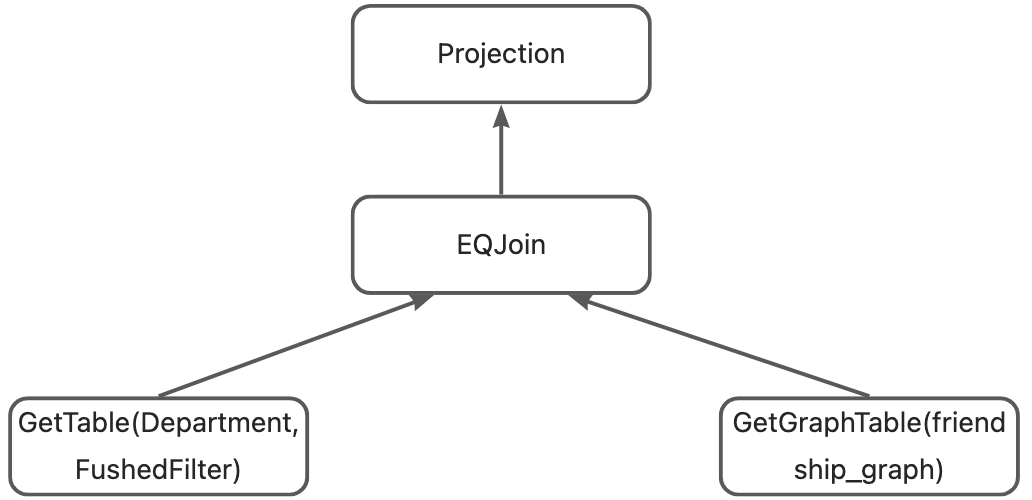
\includegraphics[width=\linewidth]{./figures/converged-logical-plan-relational-optimized.png}
        \caption{Outer query plan after Optimization.}
        \label{fig:relational-plan-optimized}
    \end{subfigure}
    \begin{subfigure}[b]{0.4\linewidth}
        \centering
        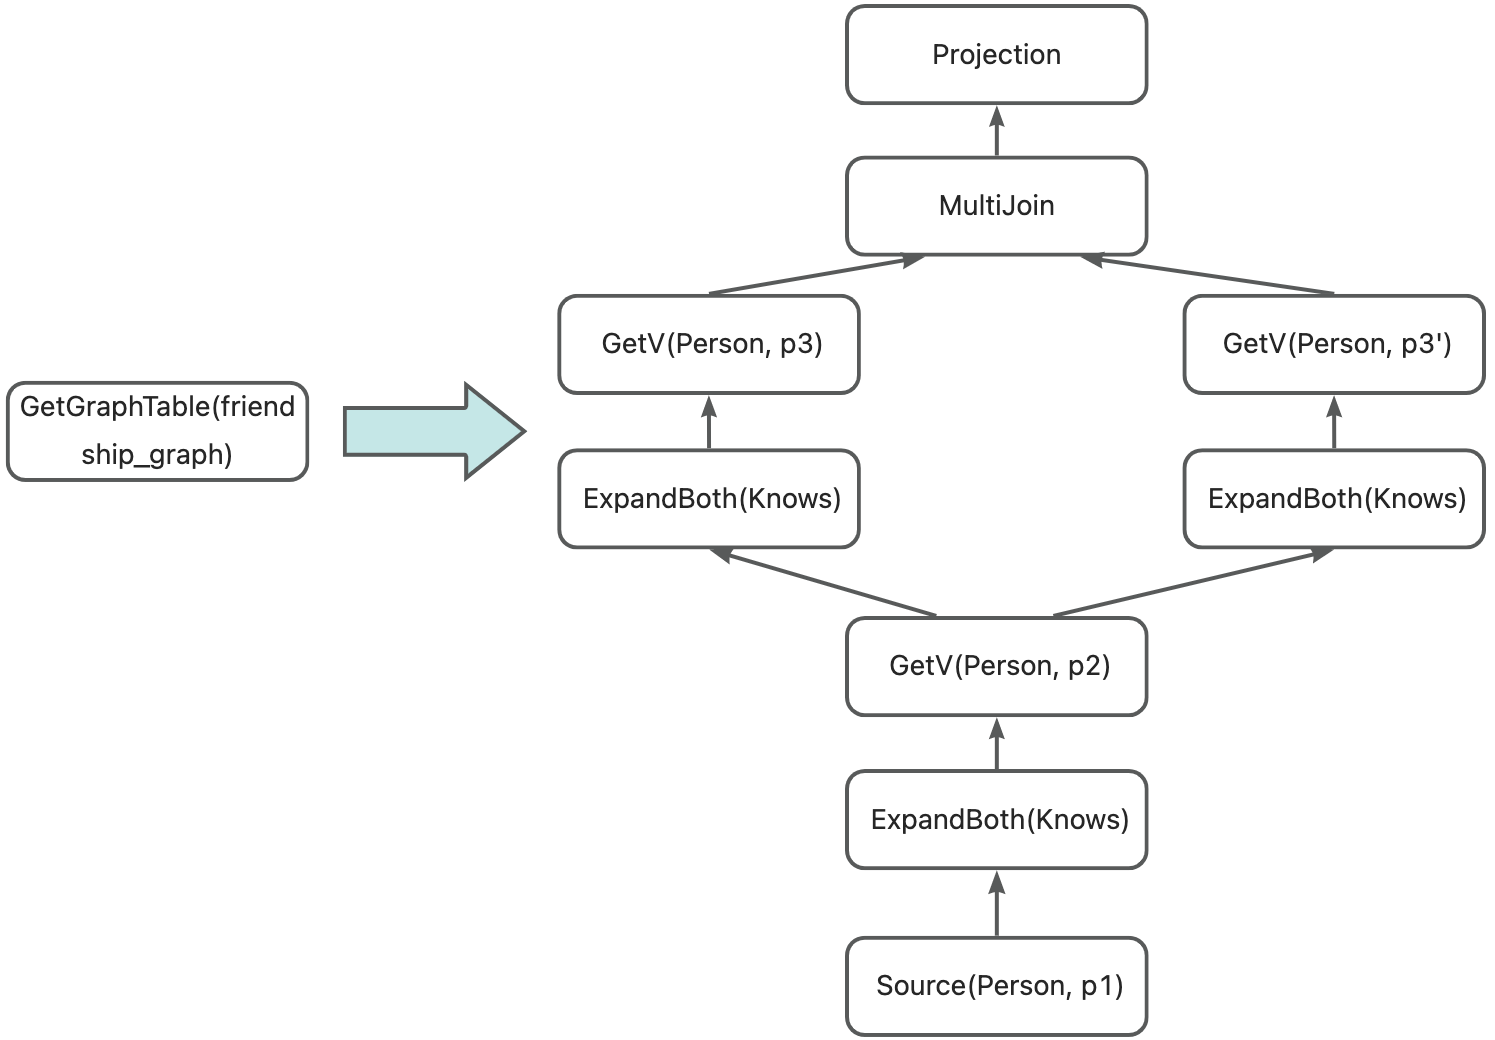
\includegraphics[width=\linewidth]{./figures/converged-logical-plan-graph-optimized.png}
        \caption{Match scanning plan after Optimization.}
        \label{fig:graph-plan-optimized}
    \end{subfigure}
    \begin{subfigure}[b]{0.5\linewidth}
        \centering
        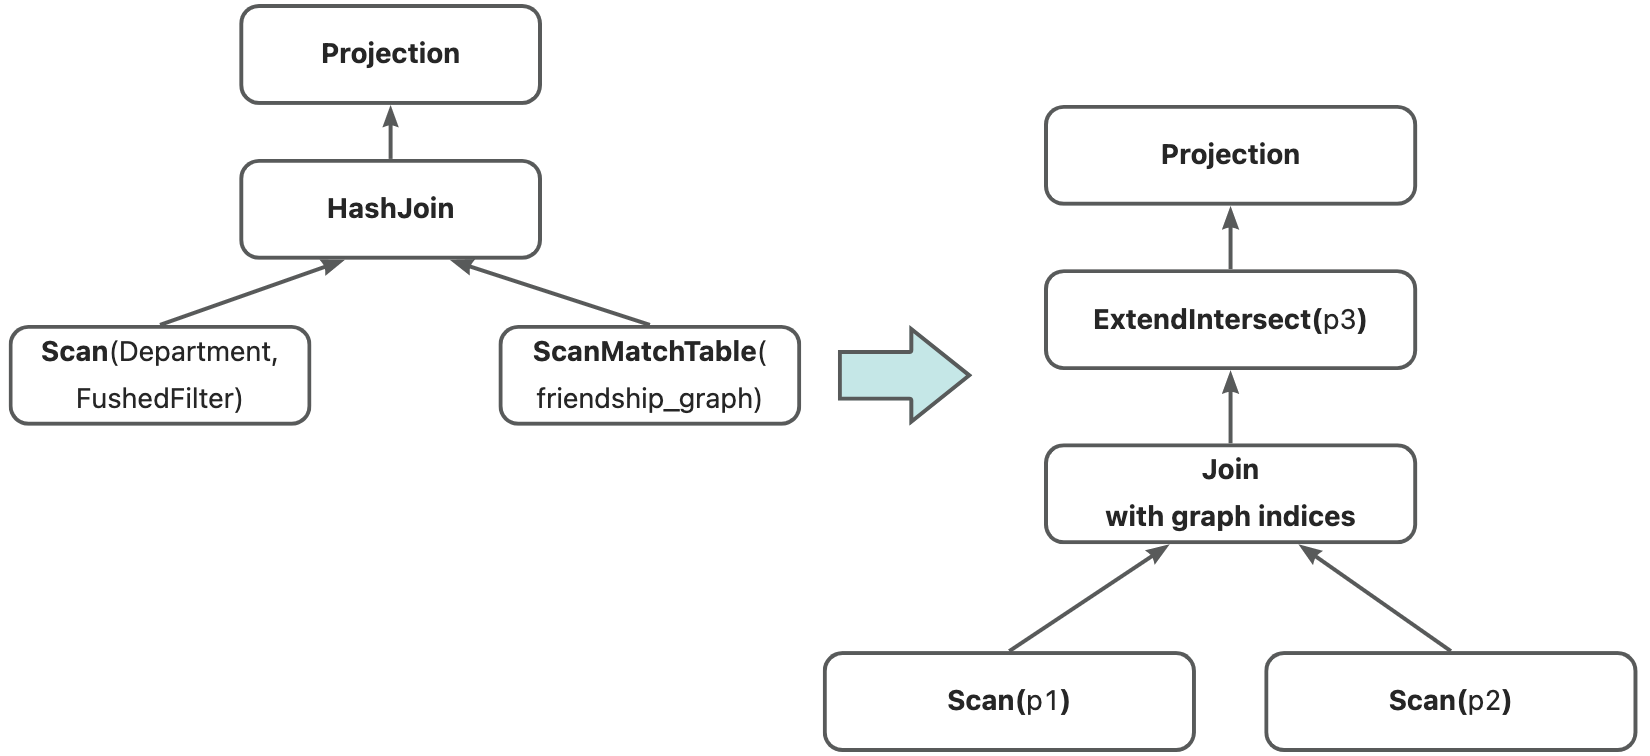
\includegraphics[width=\linewidth]{./figures/converged-physical-plan.png}
        \caption{Obtained Optimial Physical Plan.}
        \label{fig:physical-plan-optimized}
    \end{subfigure}
    \caption{An example of query opitmization.}
    \label{fig:query-grtree-example}
\end{figure*}



The above process of query processing is illustrated with the following example.

\begin{example}
    \label{example:framework}
    Given a relational database with tables as follows,
    \begin{equation*}
        \begin{split}
            & \textit{Person = (\underline{id}, name, dept\_id)} \\
            & \textit{Knows = (\underline{id1}, \underline{id2})} \\
            & \textit{Department = (\underline{dept\_id}, dept\_name)}, \\
        \end{split}
    \end{equation*}
    suppose we are going to find three persons satisfying: 
    (1) These three persons know each other;
    (2) At least two of them are from the department of computer science.
    The SPJM query can be illustrated as shown in Fig.~\ref{fig:example-operator-tree}.
    
    In relational matching algebra, the SPJM query can be expressed as follows:
    Firstly, to obtain the triangles, the pattern $\mathcal{P}_{\triangle}$ is
    \begin{lstlisting}
        (p1:Person)-[:Knows]-(p2:Person),
        (p2)-[:Knows]-(p3:Person),
        (p1)-[:Knows]-(p3)
    \end{lstlisting}
    Then, to get the relational table that records the three person and their departments, the algebra expression is 
    \begin{equation*}
        \begin{split}
            \widehat{R}_{graph} = & \pi_{p1.name\rightarrow pn1, p1.dept\_id \rightarrow dept1,p2.name\rightarrow pn2, p2.dept\_id \rightarrow dept2,} \\
            & _{p3.name\rightarrow pn3, p3.dept\_id \rightarrow dept3}(\mathcal{M}(GR, \mathcal{P}_{\triangle})),
        \end{split}
    \end{equation*}
    where $GR$ is a graph relation with only one tuple, and each attribute of the tuple is a vertex or an edge.
    The vertices correspond to rows in table Person and edges correspond to rows in table Knows.

    Finally, to obtain the triangles of persons with at least two persons from the department of computer science, the algebra expression is
    \begin{equation*}
        \begin{split}
        \pi_{pn1, pn2, pn3}
        (& \sigma_{dept.dept\_name = \text{`Computer Science'}}( \\ 
        & dept \Join_{dept1=dept.dept\_id \land dept2=dept.dept\_id} \widehat{R}_{graph})).
        \end{split}
    \end{equation*}

    Based on the above algebra expressions, the match scanning plan is shown in Fig.~\ref{fig:converged-logical-plan-graph} and the outer query plan is shown in Fig.~\ref{fig:converged-logical-plan-relational}.
    
    Then, optimization modules in the optimization layer are applied to optimize the plans.
    The optimized plans are shown in Fig.~\ref{fig:relational-plan-optimized} and Fig.~\ref{fig:graph-plan-optimized}.
    Moreover, the finally obtained optimal physical plan is shown in Fig.~\ref{fig:physical-plan-optimized}.
\end{example}

